\section{АЛГОРИТМІЧНЕ ЗАБЕЗПЕЧЕННЯ ПРОЦЕСУ СТВОРЕННЯ КОРПОРАТИВНОЇ СИСТЕМИ}

\subsection{Проектування системи}
На початку розробки будь-якого програмного продукту слід значну увагу приділити проектування системи, адже саме від цього буде залежати легкість і правильність подальшої розробки системи, її підтримка і удосконалення.
Саме тому проектування визначає основну складову програмного забезпечення. 
Необхідні пункти для успішного запуску  продукту:
\begin{enumerate}
	\item побудова UML діаграми класів;
	\item побудова діаграми відношень між об'єктами;
	\item проектування бази даних;
	\item створення макетів майбутнього інтерфейсу;
	\item чітке розмежування модулів системи і їх взаємодія і тому подібне.
\end{enumerate}

\par Як було згадано вище, перш за все слід розробити діаграму класів, показати всі взаємовідношення між об'єктами, їх роль у системі та загальну взаємодію.
\subsubsection{Модель архітектури системи}
Вся робота системи організована за принципом MVC шаблону.
\par Модель-вид-контролер -- архітектурний шаблон, який використовується під час проектування та розробки програмного забезпечення.
\par Як показана на рисунку \ref{pic:mvc} цей шаблон поділяє систему на три частини: модель даних, вигляд даних та керування. Застосовується для відокремлення даних (модель) від інтерфейсу користувача (вигляду) так, щоб зміни інтерфейсу користувача мінімально впливали на роботу з даними, а зміни в моделі даних могли здійснюватися без змін інтерфейсу користувача.

\begin{center}
		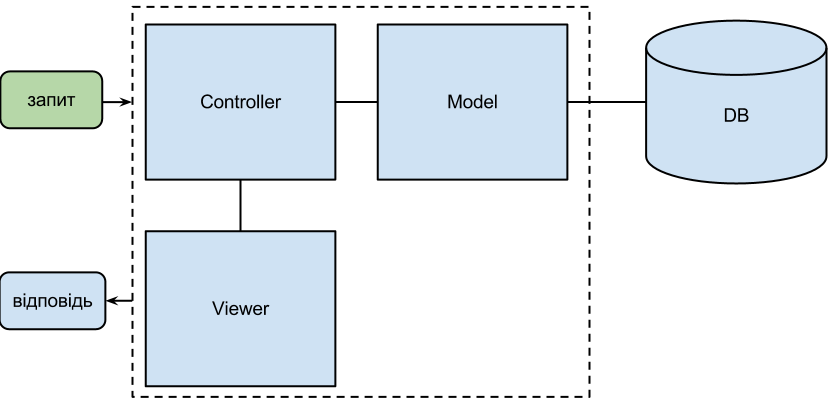
\includegraphics[width=1.00\textwidth]{mvc.png}
		\captionof{figure}{Архітектура MVC}\label{pic:mvc}
\end{center}

\par Головна мета використання даного шаблону -- гнучкий дизайн програмного забезпечення, який повинен полегшувати подальші зміни чи розширення програм, а також надавати можливість повторного використання окремих компонент програми. 
Крім того використання цього шаблону у великих системах призводить до певної впорядкованості їх структури і робить їх зрозумілішими завдяки зменшенню складності.

\par Як згадувалося раніше, архітектурний шаблон Модель-Вид-Контролер (MVC) поділяє програму на три частини. У тріаді до обов'язків компоненту Модель (Model) входить зберігання даних і забезпечення інтерфейсу до них. Вигляд (View) відповідальний за представлення цих даних користувачеві. Контролер (Controller) керує компонентами, отримує сигнали у вигляді реакції на дії користувача, і повідомляє про зміни компоненту Модель. Така внутрішня структура в цілому поділяє систему на самостійні частини і розподіляє відповідальність між різними компонентами.
\par MVC поділяє цю частину системи на три самостійні частини: введення даних, компонент обробки даних і виведення інформації. Модель, як вже було відмічено, інкапсулює ядро даних і основний функціонал з їх обробки. Також компонент Модель не залежить від процесу введення або виведення даних. Компонент виводу Вигляд може мати декілька взаємопов'язаних областей, наприклад, різні таблиці і поля форм, в яких відображається інформація. У функції Контролера входить моніторинг за подіями, що виникають в результаті дій користувача (зміна положення курсора миші, натиснення кнопки або введення даних в текстове поле).
Зареєстровані події транслюються в різні запити, що спрямовуються компонентам Моделі або об'єктам, відповідальним за відображення даних. Відокремлення моделі від вигляду даних дозволяє незалежно використовувати різні компоненти для відображення інформації. Таким чином, якщо користувач через Контролер внесе зміни до Моделі даних, то інформація, подана одним або декількома візуальними компонентами, буде автоматично відкоригована відповідно до змін, що відбулися.


\subsection{Проектування бази даних}
База даних базується на СКБД MySQL - відкритій системі. Взаємозв'язок із користувачами відбувається через Модель системи (див. рис. \ref{pic:mvc}). В базі містяться всі необхідні дані. Паролі користувачів зберігаються у шифрованому вигляді.

\subsubsection{InnoDB механізм}
\par InnoDB це потужний механізм (рушій) для зберігання даних, розроблений фінською компанією Innobase Oy, яка була придбана в 2006 році концерном Oracle Corporation.
\par Поширюється за ліцензією GNU General Public License. Є у всіх нових версіях MySQL, і, починаючи з версії 5.5 для MySQL механізм за замовчуванням.
\par Застосування InnoDB дозволяє використання базою даних таких функцій, як транзакції, зовнішні ключі. Він також сумісний з ACID.
\par У цьому рушії є два способи для зберігання даних: файл або група файлів, загальних для всіх баз даних і таблиць, або один файл даних для кожної таблиці. Інші важливі особливості InnoDB: блокування на рівні рядків, можливість стиснення даних, і MVCC.

\subsubsection{Архітектура бази даних}
\par Головною одиницею бази даних є таблиця яка відповідає за дані користувачів, адже саме від неї залежать більшість таблиць. Для прикладу це повідомлення, чи завдання.
\par Для зв'язку між таблицями використовуються зовнішні ключі. Зовнішній ключ це -- атрибут (набір атрибутів) в деякому відношенні R, який відповідає первинному ключу іншого відношення або того ж таки відношення R.
\par Ці відношення представляється у вигляді відношень. Розділяють три види відношень:
\begin{enumerate}
	\item Багато-до-багато (n:m)
	\item Один-до-багато (1:m)
	\item Один-до-одного (1:1)
\end{enumerate}
\par Багато-до-багатьох SQL відносин використовується, коли деяка невизначена кількість рядків (n) в таблиці пов'язані з невизначеною кількістю рядків (m), які зберігаються в іншій таблиці. Це називається: m:m відносини, тому що (n) рядків у першій таблиці, відносяться до (m)) рядків в іншій.
\par Потрібно бути впевненим, що використовується кількість рядків строго більше ніж одиниця, тому що у випадку із одиницею слід використовувати відношення один-до-багатьох (1:n).
\par Розглянемо приклад, який зберігає країни в одну таблицю і мови в іншу таблицю. Є країни в світі, де більш ніж одна офіційний мова, і відповідно є випадки коли говорять одною мовою більш ніж в одній країні. Саме для цього призначене відношення багато-до-багатьох. Приклад приведено на рисунку:
\begin{center}
		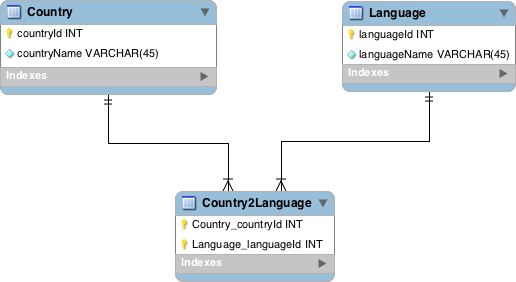
\includegraphics[width=1.00\textwidth]{many-to-many.png}
		\captionof{figure}{Відношення багато-до-багато}
\end{center}

\par Один-до-багатьох
\par Один-до-одного


\begin{center}
		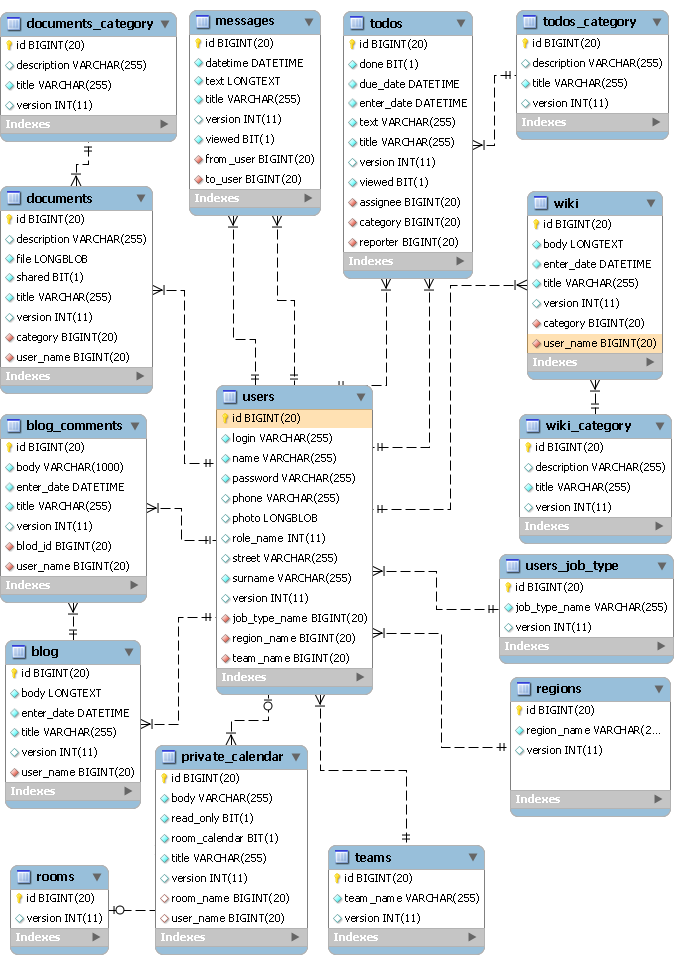
\includegraphics[width=1.00\textwidth]{db_schema.png}
		\captionof{figure}{Загальна схема структури бази даних}
\end{center}





\subsection{Структура проекту}

\begin{center}
		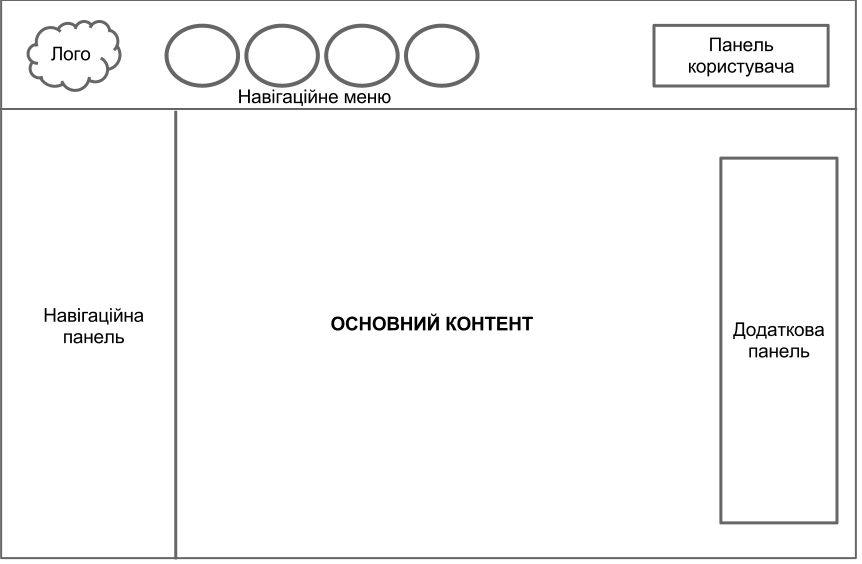
\includegraphics[width=1.00\textwidth]{mockup_mainpage.png}
		\captionof{figure}{Макет майбутнього сайту}
\end{center}


\begin{center}
		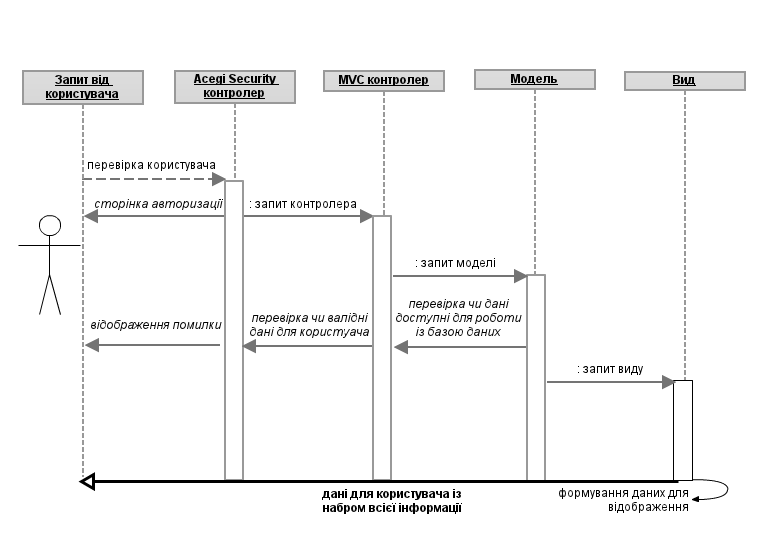
\includegraphics[width=1.00\textwidth]{sequence_diagram.png}
		\captionof{figure}{Діаграма відношення запиту користувача до роботи сервера}
\end{center}


\subsection{Авторизація і аутентифікація}
Основою будь-якої корпоративної системи є можливість використання системи управління користувачами.
Тому слід розробити повний цикл взаємодії користувачів. Сюди повинні бути включені наступні важливі аспекти:
\begin{enumerate}
	\item можливість авторизації користувачів;
	\item ролі користувачів;
	\item зберігання даних у закодованому вигляді;
	\item чіткий розподіл прав користувачів;
	\item легка взаємодія між користувачами;
	\item можливість інтеграції із іншими сервісами системи.
\end{enumerate}

Кожний працівник (він же користувач системи) повинний мати безперебійний доступ до свого профілю в будь-який час.
Авторизація повинна бути реалізована інтуїтивно зрозуміло для кожного користувача і легко доступна.
Управління користувачами буде реалізовано через адміністративну панель, доступ до якої будуть мати тільки користувачі певної групи.

\subsubsection{Алгоритм авторизації користувачів}
Загальний алгоритм авторизації полягає в перевірці даних користувача і повернення від серверу сформованих даних.
\par Сервер спочатку 

Слід виділити наступні групи користувачів:
\begin{enumerate}
	\item Адміністратори;
	\item Відділ кадрів;
	\item Користувач без особливих прав доступу.
\end{enumerate}

\par Розглянемо більш детально кожну групу. 
\par Група \"Адміністратор\" передбачає повний контроль над ресурсом. 


